\documentclass[11pt,a4paper,review]{siamart220329}
%\usepackage[margin=0.5in]{geometry}
%\documentclass[11pt,a4paper]{siamart171218}
\newcounter{savecntr}
\newcounter{restorecntr}

\usepackage{braket}
\usepackage[utf8]{inputenc}
\usepackage[english]{babel}

\usepackage{tikz}
\usetikzlibrary{shapes.geometric}

\usepackage{graphicx}
\usepackage{fancyhdr}
\usepackage{dsfont}
\usepackage{stmaryrd}
\usepackage{bbm}

\usepackage{amsfonts}
\usepackage{amssymb}
%\usepackage{amsthm}

\usepackage{amsmath}
\DeclareMathOperator*{\argmax}{arg\,max}
\DeclareMathOperator*{\argmin}{arg\,min}
\usepackage{amsfonts}
\usepackage{amssymb}
\usepackage{mathtools}
\usepackage{enumitem}

\usepackage{xcolor}
\newcommand{\tianyi}[1]{{\color{red}{TS: #1}}}

\usepackage{mathrsfs}


\usepackage{overpic} 

\usepackage{algorithm}
\usepackage[noend]{algpseudocode}

\usepackage{mathtools,booktabs}
\DeclarePairedDelimiter\ceil{\lceil}{\rceil}
\DeclarePairedDelimiter\floor{\lfloor}{\rfloor}
\algrenewcommand\algorithmicrequire{\textbf{Input:}}
\algrenewcommand\algorithmicensure{\textbf{Output:}}

\usepackage{varwidth}

\usepackage[title]{appendix}

\newcommand{\ttrank}{{\rm rank}^{\rm TT}}
\newcommand{\mlrank}{{\rm rank}^{\rm ML}}
\newcommand{\cprank}{{\rm rank}^{\rm CP}}
\newcommand{\ttsto}{p^{{\rm TT}}}
\newcommand{\mlsto}{p^{{\rm ML}}}
\newcommand{\cpsto}{p^{{\rm CP}}}
\newcommand{\rank}{{\rm rank}}
\newcommand{\lex}{<_{\rm lex}}
\newcommand{\lexeq}{\le_{\rm lex}}
\newtheorem{example}{Example}[section]
\newcommand{\ylrev}[1]{{\color{red}{[#1]}}}
%\usepackage{cite}
\usepackage{color}

\usepackage[backend=bibtex]{biblatex}
\bibliography{references}

\title{Distributed memory parallel tensor decomposition in Tensor-train format\thanks{Submitted to the editors \today.}}
\author{Tianyi Shi\thanks{Scalable Solvers Group, Lawrence Berkeley National Laboratory, Berkeley, CA 94720. (\email{tianyishi@lbl.gov})}
\and Daniel Hayes\thanks{Department of Mathematical Sciences, University of Delaware, Newark, DE 19716. (\email{dphayes@udel.edu})}
\and Jingmei Qiu\thanks{Department of Mathematical Sciences, University of Delaware, Newark, DE 19716. (\email{jingqiu@udel.edu})}}
\headers{Distributed memory Tensor-train decomposition}{T. Shi, D. Hayes, and J. Qiu}

\begin{document}
\newcommand{\R}[0]{\mathbb{R}}
\newcommand{\C}[0]{\mathbb{C}}
\maketitle

\begin{abstract}
The tensor-train (TT) format is a data-sparse tensor representation commonly used in high-order correlation functions, molecular simulations, and data science. In this paper, we propose subtensor parallel TT decompositons, a distributed memory framework for parallel TT factorization algorithms. This framework is based on multidimensional processor partitioning schemes, and we design two algorithms within the framework: (1) Data-driven subtensor parallel TT cross approximation, and (2) Analytical subtensor parallel TT sketching. We provide communication and scaling analysis, and numerical results for each method. For example, on a medical dataset with..., our parallel TT cross can achieve..., improving upon... from previous algorithms.
\end{abstract}

\begin{keywords}
Tensor-Train, parallel computing, low numerical rank, dimension reduction, data analysis
\end{keywords}

\begin{AMS}
15A69, 65Y05, 65F55
\end{AMS}

\section{Introduction}\label{sec:introduction}
The success and development of computing machines in the past few decades have allowed researchers to deal with large scale and high dimensional data easily. Typically, these data sets are stored as multidimensional arrays called tensors~\cite{kolda2009tensor}, and a general tensor $\mathcal{X} \in \C^{n_1\times\cdots \times n_d}$ requires a storage cost of $\prod_{j=1}^d n_j$ degrees of freedom. This scales exponentially with the dimension $d$, and is often referred to as ``the curse of dimensionality". Therefore, data-sparse tensor formats such as canonical polyadic (CP)~\cite{hitchcock1927expression}, Tucker~\cite{de2000multilinear}, tensor-train (TT)~\cite{oseledets2011tensor}, and tensor networks~\cite{evenbly2011tensor} with more complex geometries have been proposed. In particular, the TT format, also known as the matrix product state (MPS) in tensor networks and quantum physics, has a memory footprint that scales linearly with respect to the mode sizes $n_j$ and dimension $d$. The TT format is widely used in applications such as molecular simulations~\cite{savostyanov2014exact}, high-order correlation functions~\cite{kressner2015low}, partial differential equations~\cite{guo2023local}, constrained optimization~\cite{dolgov2017low,benner2020low}, and machine learning~\cite{vandereycken2022ttml,novikov2020tensor}. Furthermore, the TT format can be incorporated with extra conditions to form special tensor representations that can capture latent data structures. For example, the quantized TT~\cite{dolgov2012fast} format is a combination of the TT format and hierarchical structures, and the tensor chain format ~\cite{espig2012note} is a result of alterations on MPS.

In practice, instead of finding an exact TT representation of a tensor $\mathcal{X}$, one aims to construct an approximation $\tilde{\mathcal{X}}$ with a low rank TT format. One major group of TT decomposition algorithms is based on variations of singular value decompositions (SVD), such as TTSVD~\cite{oseledets2011tensor} and TT sketching~\cite{che2019randomized}, and has a guarantee that with stability and high probability,
\begin{equation}
\| \mathcal{X} - \tilde{\mathcal{X}} \|_F \leq \epsilon \| \mathcal{X} \|_F, \qquad \|\mathcal{X}\|_F^2 = \sum_{i_1=1}^{n_1} \cdots \sum_{i_d = 1}^{n_d} |\mathcal{X}_{i_1,\ldots,i_d}|^2,
\label{eq:FrobeniusNorm}
\end{equation}
where $0\leq\epsilon<1$ is an accuracy tolerance~\cite{grasedyck2013literature,hackbusch2012tensor}. Another category of TT approximation algorithms is to build $\tilde{\mathcal{X}}$ iteratively with heuristic approaches, such as TT alternating least squares~\cite{holtz2012alternating} and TT-cross~\cite{oseledets2010tt}. Although we do not have theoretical guarantees for convergence or convergence rates, these methods can have good performance in certain scenarios. Particularly, TT-cross is a data-based algorithm, with small complexity cost and especially suitable for giant dataset.

In order to exploit modern computing architectures, researchers have proposed various methods for tensor decomposition in CP~\cite{li2017model,smith2015splatt}, Tucker and hierarchical Tucker~\cite{austin2016parallel,grasedyck2019parallel,ballard2020tuckermpi,kaya2016high}, and TT~\cite{shi2023parallel,grigori2020parallel,chen2017parallelized,wang2020adtt,dolgov2020parallel} format. In addition, tensor operations in TT format, including addition and multiplication~\cite{daas2022parallel}, contraction~\cite{solomonik2014massively}, and recompression~\cite{al2023randomized} can be executed in parallel as well. The major challenge we address in this paper is to construct an approximation $\tilde{\mathcal{X}}$ in a TT format from large $\mathcal{X}$ with distributed memory parallelism. This allows one to partition $\mathcal{X}$ into smaller blocks so that each processor handles a significantly smaller chunk of data. Furthermore, with a successful distributed memory design, all processors can execute individual shared memory parallel algorithms and minimize communications with each other, leading to efficient computational and storage consumption.

In this paper, we build a distributed memory framework based on subtensors and use it for TT decomposition. A subtensor is a multilinear generalization of a submatrix, and has been used in the matricized-tensor times Khatri-Rao product (MTTKRP)~\cite{ballard2018, ballard2020}, hierarchical subtensor decomposition~\cite{ehrlacher2021}, parallel Tucker decomposition~\cite{ballard2020tuckermpi}, and parallel TT decomposition~\cite{shi2023parallel}. With this framework, one can choose any tensor algorithm and instruct all subtensors to execute it independently. In the end, results on subtensors are gathered to form the outcome of the entire tensor. For the remainder of this paper, we call this subtensor parallelism, as opposed to dimension parallelism in past literature. Dimension parallel algorithms partition computations with respect to the dimension of the tensor, and thus the number of processors used actively is limited even in the distributed memory setting. In subtensor parallelism, we construct a multidimensional processor grid for subtensor partitioning, and we can run dimension parallel algorithms in the shared memory setting on each processor as a bonus. This enables us to derive explicit bounds on the bandwidth and communication costs corresponding to the selected tensor algorithms. In particular, we focus on two algorithms:
\begin{itemize}[leftmargin=*,noitemsep]
\item \textbf{Subtensor Parallel TT Cross}: In many applications such as numerical integration in quantum mechanics~\cite{meyer1990multi} and inverse problems with uncertainty~\cite{stuart2010inverse}, and data analysis in statistical science~\cite{mccullagh2018tensor} and machine learning~\cite{rabanser2017introduction}, tensors are often formed without an exact formula and can be extremely sparse. In these cases, researchers develop TT cross~\cite{oseledets2010tt} and dimension parallel TT cross~\cite{dolgov2020parallel} for data centric TT approximation. In~\cref{sec:subTTcross}, we extend the pivot selection algorithm in dimension parallel TT cross on the entire tensor to local pivot selection on subtensors, and show the nestedness of the pivots still hold. Then, we can apply dimension parallel TT cross on each subtensor in a shared memory setting, and we can show our algorithm can obtain a comparably good approximation with minimal communication.

\item \textbf{Subtensor Parallel TT Sketching}: In~\cite{shi2023parallel}, the authors introduce a dimension parallel TTSVD algorithm, together with a randomized dimension parallel TT sketching. They use the idea of subtensors in practice, and apply the dimension parallel algorithms on the sub-blocks. However, since they focus on streaming tensors, subtensors are passed to the processors whenever one becomes idle. In other words, there does not exist a regular pattern of the possession of the subtensors to the processors, so analysis of the subtensor parallel TT sketching algorithm becomes impossible. In~\cref{sec:subComm}, we apply the multidimensional processor grid to parallel TT sketching, and derives bounds of computational, storage, and communication costs.
\end{itemize}

We implement our parallel algorithms with both distributed and shared memory parallelism in Python. Particularly, we use MPI4Py for distributed memory setup, which is a Python framework of the message passing interface (MPI). In addition, we use Numpy for linear algebra operations to optimize our codes, which is a Python wrapper for well-established linear algebra packages such as BLAS and LAPACK. The remaining of the manuscript is organized as follows.~\Cref{sec:background} reviews some necessary tensor notations and the TT format with existing serial and parallel algorithms. In~\cref{sec:subTTcross}, we introduce the new subtensor parallel TT cross algorithm. Then, we provide scalability and complexity analysis of distributed memory parallel TT cross and sketching in the subtensor framework in~\cref{sec:subComm}. Finally, we demonstrate their performance on synthetic and real-world datasets in~\cref{sec:NumericalExamples}. 



\section{Tensor notations, TT format, and decomposition algorithms} \label{sec:background}
In this section, we review some tensor notations, the TT format for low rank tensor approximations, and some TT decomposition algorithms. Throughout this paper, we aim to obtain an approximation $\tilde{\mathcal{X}}$ with low TT ranks of a given tensor $\mathcal{X}$. Whenever possible, we further require the approximation satisfies~\cref{eq:FrobeniusNorm} for some $0 < \epsilon < 1$.

\subsection{Tensor notation} \label{sec:notation}
We use lower class letters for vectors, capital letters for matrices, and calligraphic capital letters for tensors. For notational simplicity, we use MATLAB-style notation to start index counting from 1, and the symbol ``:" in indexing. This includes using $a\!:\!b$ to represent the inclusive index set $\{a,a+1,\ldots,b\}$, and a single ``:" to represent all the indices in that dimension from start to end. For example, if $\mathcal{Y} \in \R^{4 \times 8 \times 10}$, then $\mathcal{Y}(:,4\!:\!6,:)$ denotes a subtensor of $\mathcal{Y}$ with size $4 \times 3 \times 10$. In addition, we use the simplified notation $A_k$ to represent the $k$th column of the matrix $A$ instead of $A(:,k)$. In this way, $(A^T)_\ell$ is used for the $\ell$th row of $A$. Finally, we use index sets for submatrix and subtensor selection. For example, $A(:,J)$ is a submatrix of $A$ with columns $A_j$ for all $j \in J$.

In addition, we use the MATLAB command ``reshape" to form a new structure according to the multi-index via reorganizing elements without changing the element ordering. For example, if $\mathcal{Y} \in \C^{n_1 \times n_2 \times n_3}$, then $Z = {\rm reshape}(\mathcal{Y},n_1n_2,n_3)$ returns a matrix of size $n_1n_2 \times n_3$ formed by stacking entries, and similarly, $\mathcal{Y} = {\rm reshape}(Z,n_1,n_2,n_3)$. The command ``reshape" is essential when flattening a tensor into matrices, which we refer to as the unfoldings of a tensor. Tensor unfoldings are fundamental to the TT format, especially in developing practical TT decomposition algorithms and bounding TT ranks. For a tensor $\mathcal{X}\in\C^{n_1\times\cdots\times n_d}$, we denote the $k$th unfolding as
\[X_k={\rm reshape}\left(\mathcal{X},\prod_{s=1}^k n_s,\prod_{s=k+1}^d n_s\right), \quad 1 \le k \le d-1.\]

\subsection{Tensor-train format} \label{sec:TT}
The TT format of a tensor $\mathcal{X}\in\C^{n_1\times \cdots \times n_d}$ comprises of $d$ TT cores, $\mathcal{G}_k \in \C^{s_{k-1} \times n_k \times s_k}$ for $1 \le k \le d$, and takes the representation
\[
\mathcal{X}_{i_1,\ldots,i_d} = \mathcal{G}_1(:,i_1,:)\mathcal{G}_2(:,i_2,:) \cdots \mathcal{G}_d(:,i_d,:), \qquad 1\leq i_k \leq n_k.
\]
In other words, each element in $\mathcal{X}$ can be computed as the product of a sequence of matrices. The vector $\pmb{s} = (s_0,\ldots,s_d)$ is referred to as the size of the TT cores, and in order for the product to be compatible, we require $s_0 = s_d = 1$. This TT representation thus has a storage cost of $\sum_{k=1}^d s_{k-1}s_k n_k$, which is linear with respect to both $d$ and $n_k$. In addition, we call a vector $\pmb{r}= (r_0,\ldots,r_d)$ the TT rank if $\pmb{r}$ contains entry-by-entry smallest possible values of the TT core size. In practice, the exact TT rank is hard to recover, so we either aim to obtain quasi-optimal TT core size from a given threshold, or build an accurate tensor approximation with small pre-selected TT core size. It is shown in~\cite{oseledets2011tensor} that ranks of tensor unfoldings bound the TT rank from above, so we hope to use $\pmb{s}$ that satisfies
\begin{equation} \label{eq:TT_trivial}
r_k \le s_k \le {\rm rank}(X_k), \quad 1 \le k \le d-1,
\end{equation}
where $\rank(X_k)$ is the rank of the $k$th unfolding of $\mathcal{X}$. Therefore, if the ranks of all $X_k$ are small, the TT format is a memory-efficient representation.~\cref{fig:TT} provides a illustration of a tensor $\mathcal{X}$ in the TT format with TT core size $\pmb{s}$, and one may visualize slices of the TT cores as ``trains".
\begin{figure}
\centering
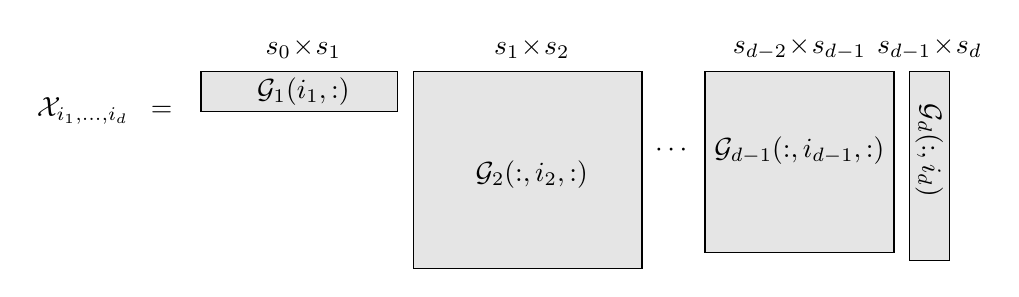
\begin{tikzpicture}
\filldraw[black] (0,-0.5) node {$\mathcal{X}_{i_1,\ldots,i_d}$};
\filldraw[black] (1,-0.5) node {$=$};
\filldraw[color=black,fill=gray!20] (1.5,0) rectangle (4,-.5);
\filldraw[black] (2.8,-0.25) node {$\mathcal{G}_1(i_1,:)$};
\filldraw[black] (2.8,0.3) node {$s_0 \! \times \! s_1$};
\filldraw[color=black,fill=gray!20] (4.2,0) rectangle (7.1,-2.5);
\filldraw[black] (5.7,-1.3) node {$\mathcal{G}_2(:,i_2,:)$};
\filldraw[black] (5.7,0.3) node {$s_1 \! \times \! s_2$};
\filldraw[black] (7.5,-1) node {$\cdots$};
\filldraw[color=black,fill=gray!20] (7.9,0) rectangle (10.3,-2.3);
 \filldraw[black] (9.1,-1) node {$\mathcal{G}_{d-1}(:,i_{d-1},:)$};
\filldraw[black] (9.1,0.3) node {$s_{d-2} \! \times \! s_{d-1}$};
\filldraw[color=black,fill=gray!20] (10.5,0) rectangle (11,-2.4);
\filldraw[black] (10.75,-1) node {\rotatebox{270}{$\mathcal{G}_{d}(:,i_{d})$}};
\filldraw[black] (10.75,0.3) node {$s_{d-1} \! \times \! s_d$};
\end{tikzpicture}
\caption{The TT format with TT core size $\pmb{s} = (s_0,\ldots,s_d)$. Each entry of a tensor is represented by the product of $d$ matrices, where the $k$th matrix in the ``train" is selected based on the value of $i_k$.}
\label{fig:TT}
\end{figure}

\subsection{TTSVD, TT sketching, and dimension parallel counterparts}
\label{sec:TTSVDalg}
If one can access all the entries of a tensor $\mathcal{X}$ at the same time, then TTSVD is the most straightforward TT decomposition algorithm, which constructs the TT cores sequentially~\cite{oseledets2011tensor}. In short, each TT core is discovered as an orthonormal (ON) basis of the column space of a reshape of the remaining information through SVD. The singular values and row space information are then grouped together to find the next TT core. Specifically, if we truncate the SVD with an accuracy of $\epsilon/\sqrt{d-1}$ in the Frobenius norm, then we obtain the TT cores of an approximation $\tilde{\mathcal{X}}$ satisfying~\cref{eq:FrobeniusNorm}. In scenarios that we cannot afford to compute SVD or we can only get elements of the tensor batch by batch, we can replace SVD by randomized SVD in TTSVD, and get the serial TT sketching algorithm~\cite{che2019randomized}. With high probability, serial TT sketching can also generate an accurate approximation $\tilde{\mathcal{X}}$.

In~\cite{shi2023parallel}, the authors use the property that column spaces of tensor unfoldings are connected to develop dimension parallel TTSVD. The algorithm calculates SVD of all tensor unfoldings simultaneously, and computes the TT cores via ON basis of column spaces of adjacent unfoldings. The result approximation can achieve the same level of accuracy as the sequential TTSVD. In addition, since only column space is essential, randomized range finders can be used to substitute SVD and the result algorithm is parallel TT sketching (see~\cref{alg:parallelTTsketching}). There are a couple of variations of parallel TT sketching with better computational and storage efficiency. For example, one can approximate both column and row space to obtain a two-sided parallel TT sketching; one can also replace the final multiplication in line 8 with an approximation so that all the tensor elements are only used once.

\begin{algorithm}
\caption{Parallel TT sketching: Given a tensor, compute an approximant tensor in TT format using sketching.}
\begin{algorithmic}[1]
\label{alg:parallelTTsketching}
\Require {A tensor $\mathcal{X} \in \C^{n_1 \times \dots \times n_d}$, TT core size $\pmb{r}$, and an oversampling parameter $p$}
\Ensure {TT cores $\mathcal{G}_1,\ldots,\mathcal{G}_d$ of an approximant $\tilde{\mathcal{X}}$}
\For {$1 \le j \le d-1$}
\State Generate $\Phi_j \in \R^{\left(\prod_{k=j+1}^d n_k\right) \times (r_j+p)}$ with i.i.d. standard Gaussian entries.
\State Calculate $S_j = X_j\Phi_j$, where $X_j$ is the $j$th flattening of $\mathcal{X}$
\State Compute a CPQR of $S_j$ to obtain $Q_j$ with ON cols and set $Q_j = Q_j(:,\!1\!:\!r_j)$.
\EndFor
\For {$1 \le k \le d-2$}
\State Calculate $W_{k+1} = Q_k^* \ {\rm reshape}(Q_{k+1}, \prod_{i=1}^k n_i ,n_{k+1}r_{k+1})$.
\State Set $\mathcal{G}_{k+1} = {\rm reshape}(W_{k+1}, r_k, n_{k+1}, r_{k+1})$.
\EndFor
\State Set $\mathcal{G}_1 = Q_1$, and $\mathcal{G}_d = Q_{d-1}^*X_{d-1}$.
\end{algorithmic}
\end{algorithm}

\subsection{Pivot selection and dimension parallel TT cross}
Algorithms based on SVD can be extremely expensive and unnecessary in many situations. For example, tensors originated from real world datasets are often large and sparse, and we often only want an approximation with an accuracy of a few significant digits. This leads to heuristic data-based methods, such as adaptive cross approximation (ACA). In summary, ACA mainly finds a ``skeleton" of original data for approximation. For example, the CUR factorization of a matrix in the form of
\[ A \approx CUR = A(:,J)A(I,J)^{-1}A(I,:), \]
where $I$ and $J$ are two index sets for selection. The key building block in ACA is new pivot selection to enrich the index sets. There are various metrics for selecting, but we focus on a greedy approach outlined in~\cite[Algorithm 2]{dolgov2020parallel}, which is computationally much cheaper than other routines such as max volume selection. Suppose we use $I_{\le k}$ and $I_{>k+1}$ to denote the selected sets of pivots for the $k$th unfolding of a tensor $\mathcal{X}$ and $\mathbb{I}_\ell$ to denote the set of all indices for dimension $\ell$ with $1 \le k \le d-1$ and $1 \le \ell \le d$, then one step of finding new pivots is described in~\cref{alg:TTcross}. Additionally, pivots selected this way can be shown to satisfy the nestedness property, which ensures that pivots found in one tensor unfolding can be carried over to subsequent unfoldings. As a result,~\cref{alg:TTcross} is automatically a dimension parallel algorithm.

\begin{algorithm}
\caption{One step of finding new pivots in TT cross.}
\begin{algorithmic}[1]
\label{alg:TTcross}
\Require {A tensor $\mathcal{X} \in \C^{n_1 \times \dots \times n_d}$, index sets $(I_{\le k}, I_{>k+1})$ containing previous pivots.}
\Ensure {New pivots $(i^*_{\le k}, i^*_{>k+1})$}
\For {$1 \le k \le d-1$}
\State Use~\cite[Algorithm 2]{dolgov2020parallel} to find $(i^*_{\le k}, i^*_{>k+1})$ on a superblock $X_k(I_{\le k-1}\times\mathbb{I}_k,\mathbb{I}_{k+1}\times I_{> k+1})$, which is seen as a submatrix of the $k$th unfolding of $\mathcal{X}$.
\EndFor
\end{algorithmic}
\end{algorithm}

\section{Subtensor parallelism for tensor-train cross approximation}
\label{sec:subTTcross}
\subsection{Submatrix parallelism for matrix cross approximation}
There are various ways to compute a matrix low rank decomposition with cross approximation. For example,~\cite[Algorithm 2]{dolgov2020parallel} provides a scheme to find a new pivot for the approximation. In this section, we aim to extend this idea to distributed memory setting. In other words, our target is to make this algorithm parallelizable, so that we can use several processors to find the new pivot with efficiency and scalability.

Suppose the matrix to be decomposed is $A$ and we have a 2D processor grid with $P = P_{\rm row}P_{\rm col}$ processors in total. Then, the processors can be labeled with $P_{k,\ell}$ with $1 \le k \le P_{\rm row}$ and $1 \le \ell \le P_{\rm col}$, which handles the submatrix $A_{k,\ell} = A(K,L)$. Here $K$ and $L$ are used to denote the row and column index sets that all processors on block row $k$ and block column $\ell$ handle respectively. If the row indices of the current selected pivots are stored in the set $I$, and column indices in $J$, then we know the matrix approximation at this step is 
\[ \tilde{A} = A(:,J)A(I,J)^{-1}A(I,:). \]
We can also find out the submatrices of $\tilde{A}$ are
\[ \tilde{A}_{k,\ell} =  A(K,J)A(I,J)^{-1}A(I,L), \]
which is essential in selecting the new pivots. Therefore, in addition to $A_{k,\ell}$, the processor $P_{k,\ell}$ also holds $A(K,J\backslash L)$ and $A(I \backslash K,L)$ to build $\tilde{A}_{k,\ell}$. This allows $\tilde{A}_{k,\ell}$ on each processor to be the same as if $\tilde{A}$ is built globally with all elements of $A$. In this way, suppose one finds a new pivot $(i^*,j^*)$ with starting random set $L$ globally on $A$ using Algorithm 2 in~\cite{dolgov2020parallel}, then the same pivot $(i^*,j^*)$ is guaranteed to be recovered on one of the submatrices if Algorithm 2 in~\cite{dolgov2020parallel} is performed on each processor and $L$ is a subset of the union of the starting random sets on each processor. After local pivots are found on each submatrix, the processors communicate to find the best pivot, and $P_{k,\ell}$ also needs to handle extra information $A(K,j^*)$ if $j^* \notin L$ and $A(i^*,L)$ if $i^* \notin K$. This distributed version of algorithm is described in Algorithm 1.

\begin{algorithm}
\caption{One step of the matrix cross interpolation algorithm on one processor.}
\begin{algorithmic}[1]
\label{alg:1}
\Require {Matrix $A$ to be decomposed, sets $(\mathcal{I},\mathcal{J})$ containing existing pivots, sets $(\mathcal{K},\mathcal{L})$ containing indices of submatrices handled by this processor.}
\Ensure {A new pivot $(i^*,j^*)$ for $A$.}
\State Perform Algorithm 2 in~\cite{dolgov2020parallel} on $A(\mathcal{K},\mathcal{L})$ to get a local pivot $(i^*_p,j^*_p)$.
\State Use \textit{Allgather} to find the best pivot $(i^*,j^*)$ on all processors.
\If $j^* \in \mathcal{L}$
\State \textit{Send} $A(\mathcal{K},j^*)$ to all processors that deal with row index set $\mathcal{K}$.
\Else
\State \textit{Receive} $A(\mathcal{K},j^*)$ from the processor that contains this data.
\EndIf
\If $i^* \in \mathcal{K}$
\State \textit{Send} $A(i^*,\mathcal{L})$ to all processors that deal with column index set $\mathcal{L}$.
\Else
\State \textit{Receive} $A(i^*,\mathcal{L})$ from the processor that contains this data.
\EndIf
\State Set $\mathcal{I} \leftarrow \mathcal{I}\cup i^*$ and $\mathcal{J} \leftarrow \mathcal{J}\cup j^*$.
\end{algorithmic}   
\end{algorithm}

\section{Tensor-train cross approximation}
The paper~\cite{dolgov2020parallel} introduces a parallel algorithm to compute tensor-train (TT) cross approximation that the parallelism is with respect to dimensionality. However, this type of parallelism has a limitation that when the tensor is low dimensional, then we cannot fully utilize the computing resources that we have. For example, when $d = 5$, then we can only use $\le 4$ MPI ranks for computation. Hence, we want to design a parallel TT cross approximation whose parallelism can allow us to allocate more processors.

We use the idea from~\cite{shi2023parallel} to assign processors to deal with subtensors. Therefore, we want to introduce the same idea for parallel TT cross approximation.

Suppose we have a tensor $\mathcal{X} \in \R^{n_1 \times \cdots \times n_d}$ and an index partitioning $P_1 \times \cdots \times P_d$ so there are $P = |P_1|\cdot\dots\cdot|P_d|$ subtensors in total, and we denote each index by $P_1^{(j)} \times \cdots \times P_d^{(j)}$ where $1 \le j \le P$. As the dimensionality parallel algorithm in~\cite{dolgov2020parallel}, we develop the new parallel algorithm based on Algorithm 5. For notational simplicity, we follow those used in~\cite{dolgov2020parallel} and let $I_{\le 1}, \dots, I_{\le d-1}, I_{>2}, \dots, I_{>d-1}$ to denote the selected subsets for the tensor unfoldings $X_1, \dots, X_{d-1}$, and $\mathbb{I}_1,\dots,\mathbb{I}_d$ to denote the set of all indices for each dimension.

In Algorithm 5, the main parallelized procedure is to find a new pivot on the superblock 
\[ X(I_{\le k-1}\times\mathbb{I}_k,\mathbb{I}_{k+1}\times I_{>k+1}), \] 
which is seen as a $r_{k-1}n_k \times n_{k+1}r_{k+1}$ matrix. In subtensor parallelism, we define 
\[ J_{\le 1}^{(j)} = I_{\le 1} \cap P_1^{(j)}, \quad J_{\le 2}^{(j)} = I_{\le 2} \cap (P_1^{(j)} \times P_2^{(j)}), \quad\dots, \] 
to indicate the set of indices in $I_{\le 1}, I_{\le 2}, \dots$ that are handled by the subtensor. Similarly we can define $J_{> 2}^{(j)},\dots$. In addition, it's straightforward to see that 
\[ P_1^{(j)} = \mathbb{I}_1 \cap P_1^{(j)}, \quad P_2^{(j)} = \mathbb{I}_2 \cap P_2^{(j)},\quad \dots. \].

In this way, we can replace $I_{\le k-1}\times\mathbb{I}_k$ by $J_{\le k-1}^{(j)}\times P_k^{(j)}$ and $\mathbb{I}_{k+1}\times I_{>k+1}$ by $P_{k+1}^{(j)}\times J_{>k+1}^{(j)}$ to represent the new set of indices significant in this subtensor. For this algorithm to work, the remaining question is to show that the set $J_{\le k}^{(j)}$ satisfy the nestedness property:
\begin{align*}
J_{\le k}^{(j)} &= I_{\le k} \cap \left(P_1^{(j)} \times\cdots\times P_k^{(j)}\right) \\
&\subset (I_{\le k-1} \times \mathbb{I}_k) \cap \left(P_1^{(j)} \times\cdots\times P_k^{(j)}\right) \\
&\subset \left[I_{\le k-1} \cap \left(P_1^{(j)} \times\cdots\times P_{k-1}^{(j)}\right)\right] \times \left( \mathbb{I}_k \cap P_k^{(j)}\right) \\
&= J_{\le k-1}^{(j)} \times P_k^{(j)}.
\end{align*}
Therefore, we have nestedness guarantee of the subtensor parallel algorithm. This means that each subtensor can find its own new pivots for each superblock, and we need to communicate between subtensors to obtain the best new pivots for the superblocks.

\section{Processor grid development for parallel tensor-train algorithms}
\label{sec:subComm}
Processor grids are often used in distributed memory programming for easier analysis of local computation and communication costs. The idea of 1D and 2D processor grids are widely adopted in numerical linear algebra, especially for vectors and matrices. In this section, we aim to use processor grids for parallel TT algorithms, mainly for TT sketching and TT cross.

For simplicity, we consider a $d$-dimensional tensor $\mathcal{X}$ whose size of each dimension is $n$. We also assume a subtensor partitioning grid to be $C \times \cdots \times C$ with $n = |C|m$, so $m$ is the size per dimension of the subtensor. It's easy to see that one can apply any $k$-dimensional processor grid to this subtensor partitioning as long as $k \le d$. However, if $|C|$ is not a multiple of $|P|$, where $P$ is the processor partitioning of any dimension, then load imbalance issue becomes more serious with smaller $k$ values. Therefore, in this section, we consider a processor grid $P \times \cdots \times P$, and assume $|C|=|P|w$ for simplicity. In this way, each processor handles $w^d$ subtensors.

\subsection{Parallel TT sketching}
We stick to the uniform size set up and assume that the TT rank we sketch for each dimension is $r$, and the oversampling parameter we use is $l$. In addition to subtensor partitioning, we also need a partition for the sketches. For dimension $j$, the sketch can be considered as a $(j+1)$-dimensional tensor of size $n \times \cdots \times n \times r$, so we need also to assign a $j$-dimensional processor grid $P \times \cdots \times P$ to it. For all possible $j$ values, we need in total
\[ |P|+|P|^2+\cdots+|P|^{d-1} = \frac{|P|^d-|P|}{|P|-1} < |P|^d \]
processors, so we can safely assign each processor we use in subtensor partitioning to handle some subsketches for a certain dimension $j$. As a result, we need two sets of processor grid for TT sketching: 1) subtensor grid, and 2) subsketch grid for all dimensions, and we need to figure out a correspondence between grids 1) and 2).

We can now do some basic and preliminary analysis for the TT sketching algorithm step by step.
\begin{enumerate}
\item Multiplication on each subtensor needs $\mathcal{O}(m^d(r+l))$ for one dimension so $\mathcal{O}(m^d(r+l)w^d(d-1))$ in total for all processors.

\item Now we consider the communication between the two types of processor grids. For dimension $j$, each processor sends at most $w^d$ subsketches, each with $m^j(r+l)$ elements. The actual send number can be smaller since there can be an overlap between the two processor grids (so that there is no need to communicate). Each processor needs to receive a total of $|C|^{d-j}w^j$ subsketches, each with $m^j(r+l)$ elements.

\item On subsketches, we need to perform a distributed memory tall-and-skinny QR~\cite{benson2013direct}. The actual algorithm is to perform QR on each subsketch, gather the information to one processor, do another QR, and scatter the results back to each subsketch. For dimension $j$, the gather and scatter processes require a communication of $w^jm^j(r+l)$ elements for each processor.

\item Finally, we need a communication across processor grids in grid 2) to perform final multiplication. This aims to communicate between different dimensions. For dimension $j$, we need to send each of $|P|^j$ processors to $|P|$. Once the multiplication is done, the results are reduced on the $P$ processors, and we can grab the TT format directly from them.

\end{enumerate}

\subsection{Parallel TT cross approximation}
For each processor, it can find new pivots $(i_{\le j}^{(p)},i_{>j}^{(p)})$ where $j$ is used to denote dimensions and $p$ is used to denote processor ID. Then, for the same $j$, the pivots, together with their error metric, are gathered together to find the best new pivot and all processors need to know this new pivot. In this gather procedure, $3|P|d$ values (column index, row index, and error metric for each processor) are communicated. After obtaining the best new pivot, each processor needs to enrich their knowledge of columns and rows in all superblocks that contain the new pivots. In total, the number of elements communicated is $mw^d\sum_{k=1}^{d-1}(r_{k-1}+r_{k+1})$, where $r$ is used to denote the size of the current set of pivots.

\section{Numerical Examples}
\label{sec:NumericalExamples}

\printbibliography

\end{document}